\documentclass{amsart}
\usepackage[pdftex]{graphicx}
\usepackage{enumerate,placeins}
\usepackage{color}
\graphicspath{{figures/}}

\title{Modeling Intervention Strategies for United States TB Control}
\begin{document}
\maketitle

{\huge \color{red} Check if first person is better.}

\section{Abstract}
A deterministic, compartmental epidemiological and economic model for US
Tuberculosis was developed, extending a model developed in 2012 by the Centers
for Disease Control and Prevention. Sensitivity analysis of this model reveals
that the percentage of foreign-born immigrants with LTBI is a highly influential
parameter. Various intervention strategies, particularly those that reduced LTBI
among foreign-born arrivals, were evaluated, and cost per case averted estimates
were found.  Additionally, a population-level, stochastic, agent-based model was
built. This model demonstrated the feasibility of using agent-based modeling in
the context of minimal population heterogeneity and provided statistical
characterization of the results of the compartmental model. Specifically, it
revealed that final population sizes were normal, with the compartmental model
sampling the mean of these distributions. 

\section{Introduction}
Epidemiological models allow public health professionals to predict and analyze
disease dynamics and intervention effectiveness. The most common examples of
such models are detereministic, compartmental, differential equation models. In
these models, the population is split between several possible health states, or
compartments, and a system of differential equations governs population flow
between the various compartments. In 2012, Hill, Becerra, and Castro implemented
a compartmental differential equaiton model of tuberculosis (TB) in the United
States (US).  Their model characterized five health states across two
subpopulations, US-born (USB) and foreign-born (FB), for a total of 10
compartments. They used this model to evaluate several possible intervention
strategies and ultimately concluded that though increasing LTBI treatment was an
effective intervention strategy, the US was unlikely to meet their stated goal
of elimination of TB in the US by 2100. Here, we present an extended Hill model
with additional tracking capabilities, such that it can now report
further granularity in the disease dynamics. Furthermore, this model also tracks
economic data in order to project the US health care system (HCS) costs due to
TB given our current policy as well as in the context of various interventions. 

{\huge \color{red} Fix this paragraph. Its not the best. \textbackslash/}

Though compartmental, differential equation models are the most common strategy
when modeling large-scale diseases at the population level, an alternative
approach is to use an agent-based model. Agent
based models provide a more nuanced view of disease spread as they provide a
more biologically accurate modeling framework; however, they are often
considered to be computationally infeasible at population level. In order to
challenge this assumption of infeasibility and provide statistical verification
of the results of the compartmental model, we implemented a stochastic,
agent-based model of US TB dynamics at the population level.

\section{Background}
\subsection{Tuberculosis}
{\huge \color{red} Add background info about TB. Latent phase, etc. I think it
makes sense to give it its own section.}
\subsection{The Hill Model}
A flowchart representation of the Hill Model is shown in
Figure~\ref{fig:hillModelSchematic}. Each compartment represents a different
possible health state with respect to TB for every US-born or foreign-born
individual, and arrows between different compartments represent possible
transitions between states.  Individuals also leave the model from all
compartments due to natural death, which is left out of the figure for clarity.

\begin{figure}[h]
  \begin{center}
    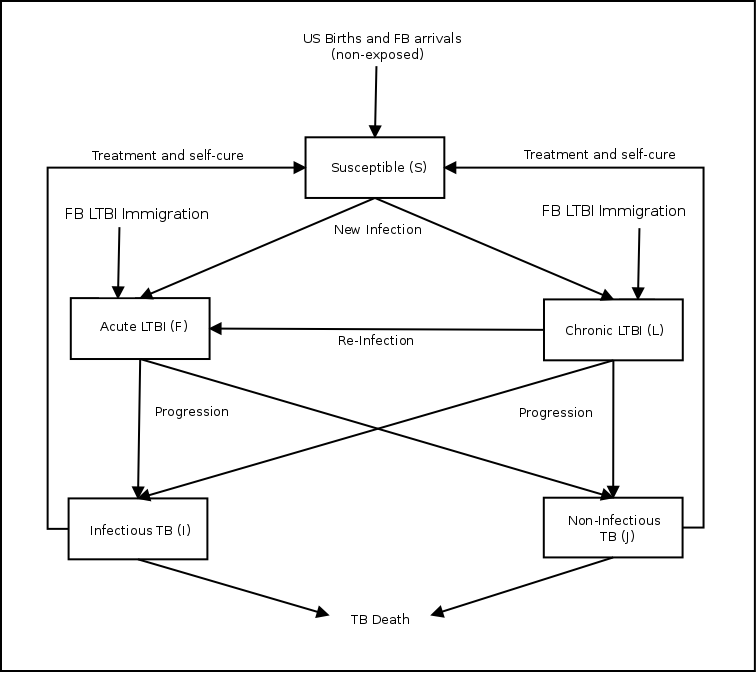
\includegraphics[scale=0.25]{figures/HillModelFlowChart.png}
  \end{center}
  \caption{Schematic of the Hill Model.}
  \label{fig:hillModelSchematic}
\end{figure}

The majority of USB and FB individuals fall into the Susceptible (S) category,
which includes everyone who is uninfected and has not been exposed to TB.  After
exposure to an individual with TB, a person in the Susceptible compartment can
develop Latent TB Infection (LTBI). Latently infected individuals are
asymptomatic and non-infectious, but have some risk of developing active TB
infection over time. To reflect the fact that real LTBI patients have a
much higher risk of developing active TB within two years of exposure, the Hill
Model splits the LTBI compartment into Acute LTBI (fast progressors) and Chronic
LTBI (slow progressors). Accordingly, individuals in the Acute LTBI compartment
have a higher risk of developing active TB than those in the Chronic LTBI
compartment. Individuals in the Chronic LTBI compartment may also be
exogenously re-infected and transition to the Acute LTBI compartment. 

Latently infected individuals may progress to one of two active TB states: Infectious TB (I) or 
Non-Infectious TB (J).  Individuals in both compartments have an increased risk of death from
active TB infection, but only individuals in the Infectious TB compartment are contagious.  
In addition, individuals in all of the infected compartments (F, L, I, J) may be treated or self-cure
themselves of their respective TB health condition.  However, in the model, treatment or self-cure from TB
does not grant immunity, and all healthy individuals are grouped in the Susceptible compartment
and may be re-infected at a later time.

{\huge\color{red} This section is good, but we may want to give a summary of the
differential equations at the end.}

\section{Methods}
\subsection{Basic Structure}
Both the Hill Model (Basic Hill Model) and our extended Model (Extended Hill
Model) were implemented in \texttt{R} as a system of differential equations,
which were solved via the $\texttt{lsoda}$ routine. The systems of differential
equations used to capture basic disease dynamics in the Basic Hill Model are
shown in Figure~\ref{fig:hillEquations}.  In the Extended Hill Model, each flow
rate equation from the Basic Hill Model was separated into its component part
and these were tracked separately. In other words, rather than tracking net flow
into various compartments, the Extended Hill Model tracks flow between all pairs
of compartments separately. Furthermore, these equations were each also supplemented to
also estimate their corresponding US HCS costs.  These equations are detailed in
the\\
{\huge\color{red} Should appendix be capitalized? What about Figure?}\\
appendix,
section~\ref{sec:extendedHillEqs}.  Historical data from 2000-2008 was used to
initialize the model, which was then run up to the year 2100.  

\begin{figure} 
  {\huge\color{red} Make this not a figure. This should definitely just be tex.}
  \begin{center}
    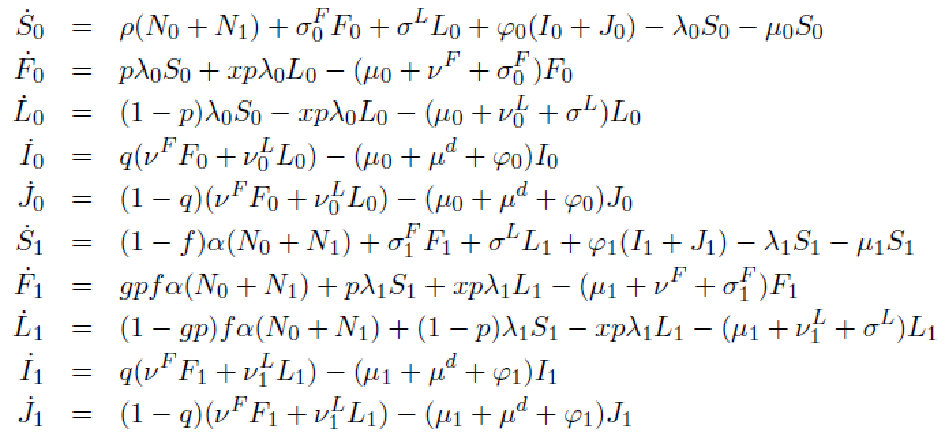
\includegraphics[scale=0.75]{figures/BasicHillEquations.pdf}
  \end{center}
  \caption{System of Differential Equations given in the Hill Model.}
  \label{fig:hillEquations}
\end{figure}

The vector variables $S_0, F_0, L_0, I_0, J_0$ contain the number of US-born
individuals in the S, F, L, I, J compartments respectively, whereas $S_1, F_1,
L_1, I_1, J_1$ contain the number of foreign-born individuals. $N_0$ and $N_1$
are the total populations of US-born and foreign-born individuals.  The
constants $\rho$ and $\alpha$ are birth rates, while $\mu_i$, and $\mu_d$ are
death rates. A complete list and descriptions of all constants used in the model
can be found in the Appendix, Section~\ref{subsec:hillConstants}.

\subsection{Additional Tracking Capabilities}
In order to refine the tracking capabilities of the Hill Model, the original
differential equations used to describe TB spread were separated into their
component parts and each section was tracked separately.
These components were made into compartments, tracked by differential equations
detailed in the appendix. Progressions into active TB due to activations of LTBI
or exogenous infection were tracked, allowing for sourced incidence data to be
generated. These equations allowed the model to track the sourced number of TB
cases, TB deaths, and natural deaths. Furthermore, the model also tracks the
sourced cost on the US HCS. The immigrating cases of LTBI (acute or chronic)
were also tracked. In the case of intervention testing, the number of cured and
untreated cases of entering LTBI were both tracked. Cured cases of LTBI
entering, TB deaths, total TB cases, and total cost were also tracked discounted
at 3\% annually. This discounting was converted to a continuous differential
equation for use within the model. In general, incidence data is calculated in
the same way in the Extended Hill Model as it was in the Basic Hill Model.

In addition, estimations of the basic reproductive number of FB or USB active,
infectious TB cases were made from a theoretical and an experimental
perspective. Experimental data were calculated by reducing the initial
FB or USB infectious TB populations by one and allowing the
model to progress otherwise as normal. The decreased number of total TB cases
seen details how many infections can be thought to be due to one infected
individual in the given population. In the agent-based model, this \emph{one}
was a true model agent whereas in the compartmental model, this decrease of
\emph{one} was a proportional decrease based on the scaled population level. 

From a theoretical perspective, the spread of TB was thought to be a geometric
series. If one infectious individual infects $x$ people annually, over the
course of $N$ years the total number of infections caused by this individual can
be approximated by the geometric series of $N$ terms with rate $x$ and initial
term $1$. In this case, $N = 100$, and the ratios for FB infectious individuals
and USB infectious individuals were obtained from <+RATIO CITATION COLIN+>
\subsection{Economic Modeling}
In order to track the US HCS economic load given the TB rates, we made the
following treatment cost assumptions. A single case of active TB was assumed to
yield a \$14,000 US HCS cost, charged immediately upon disease contraction. This
cost is the weighted mean of the costs of cases requiring hospitalization
(happening 49\% of the time) and cases not requiring hospitalization (51\%).
These cost estimates were found in <+DYLAN COST STUDY CITATION+>. LTBI treatment
costs were given by \$468.00 US HCS cost, charged immediately upon successful
treatment. These estimates were calculated based on the cost of a successfull
treatment, and the typical adherence and efficacy of said treatment <+DYLAN COST
STUDY CITATION, ADHERENCE CITATION+>. It is important to note that the charging
assumptions are different for treatment of active TB as opposed to treatment of
latent TB. In particular, cases of active TB imply a cost immediately upon
disease contraction, whereas latent TB costs are charged only upon successful
treatment. The motivation for this distinction is that active TB treatment is
mandated by the US for all known cases and, further, most treatment costs are
incurred at the beginning of the treatment cycle. As such, charging for every
known case, immediately at contraction is a well motivated assumption. On the
other hand, latent TB is only rarely treated in discovered cases and the costs
are more evenly distributed. Furthermore, the choice to charge only upon
successful treatment yields a more conservative estimate of the success of any
intervention analyzed. 

Cost data were separately tracked due to incoming active TB costs stemming from
activation of LTBI vs exogenous reinfection. These data were modelled as
additional compartments and also solved by $\texttt{lsoda}$.  Given the
uncertainty in measurments of LTBI treatment cost, extensive sensitivity
analysis was performed on this parameter relative to final cost outcomes. In
addition to US HCS cost, the system was implemented so as to also track
projected intervention implementation cost, given user-inputted parameters
relating to various possible intervention cost strategies. The extended Hill
Model was used to track the effect of many interventions tested by the Hill
Model. In particular, the intervention strategy of curing entering cases of LTBI
proved very promising and elimination year, final cost, and cost per case
averted were tracked for various levels of entering LTBI cure rate. The
interventions were implemented so as to take effect during the year 2013 and run
to 2100. The numerical DE solver $\texttt{lsoda}$ used was run with a time step
of $0.8$. Sensitivity analysis was performed on this parameter and reducing the
time step was shown to have minimal effect on final size or cost values.

\subsection{Agent Based}
The population level agent based model was implemented in several ways. Early
implementations were built in \texttt{Netlogo} and \texttt{Java}, but final
implementations were constructed in $\texttt{C++}$. Probabilites of agent
progression between various health states were computed given rates in the hill
model and a variety of integration approximations. The model maintained
individual records for every individual with LTBI or active TB. Susceptible
individuals were not modelled as agents; instead, a binomial distribution was used to
probabilistically determine the number of new infections each time step.
Similarlly, the number of new immigrants each time step was chosen from a
probability distribution. We collected final population distribution data via
<+NUMBER OF RUNS 2160+> runs with each agent in the model truly representing one
infected individual and a time step of $0.01$.  These data were analyzed in $R$.
This model was also made to track deaths, total TB cases, and infection sources,
as well as economic data. These data were consistently normal and matched the
deterministic model. 

Further implementations of the \texttt{C++} model were made that deviated from
the basic Hill Model. Specifically, the acute latent compartment in the basic
Hill Model is a vestigal necessity of compartmental modeling and not reflective
of the biology of tuberculosis. As such, an agent based model was implemented
that more closely respects the biology of tuberculosis. Results from this model
were also normal and did not differ significantly from the strict Hill model. 

\section{Results}
\subsection{Basic Population Breakdown}
The additional tracking capabilities offered several key insights into US TB
dynamics. Figure~\ref{fig:incPlotSourced} shows the yearly incidence of US TB, broken
down into infection source. It can be seen that the majority of the US TB load
is driven by activations of FB LTBI, followed by USB LTBI activations. This data
further agrees with the conclusions drawn by Hill, Becerra, and Castro about the
necessity of LTBI treatment in any effective intervention strategy. 
\begin{figure}[h]
  \begin{center}
    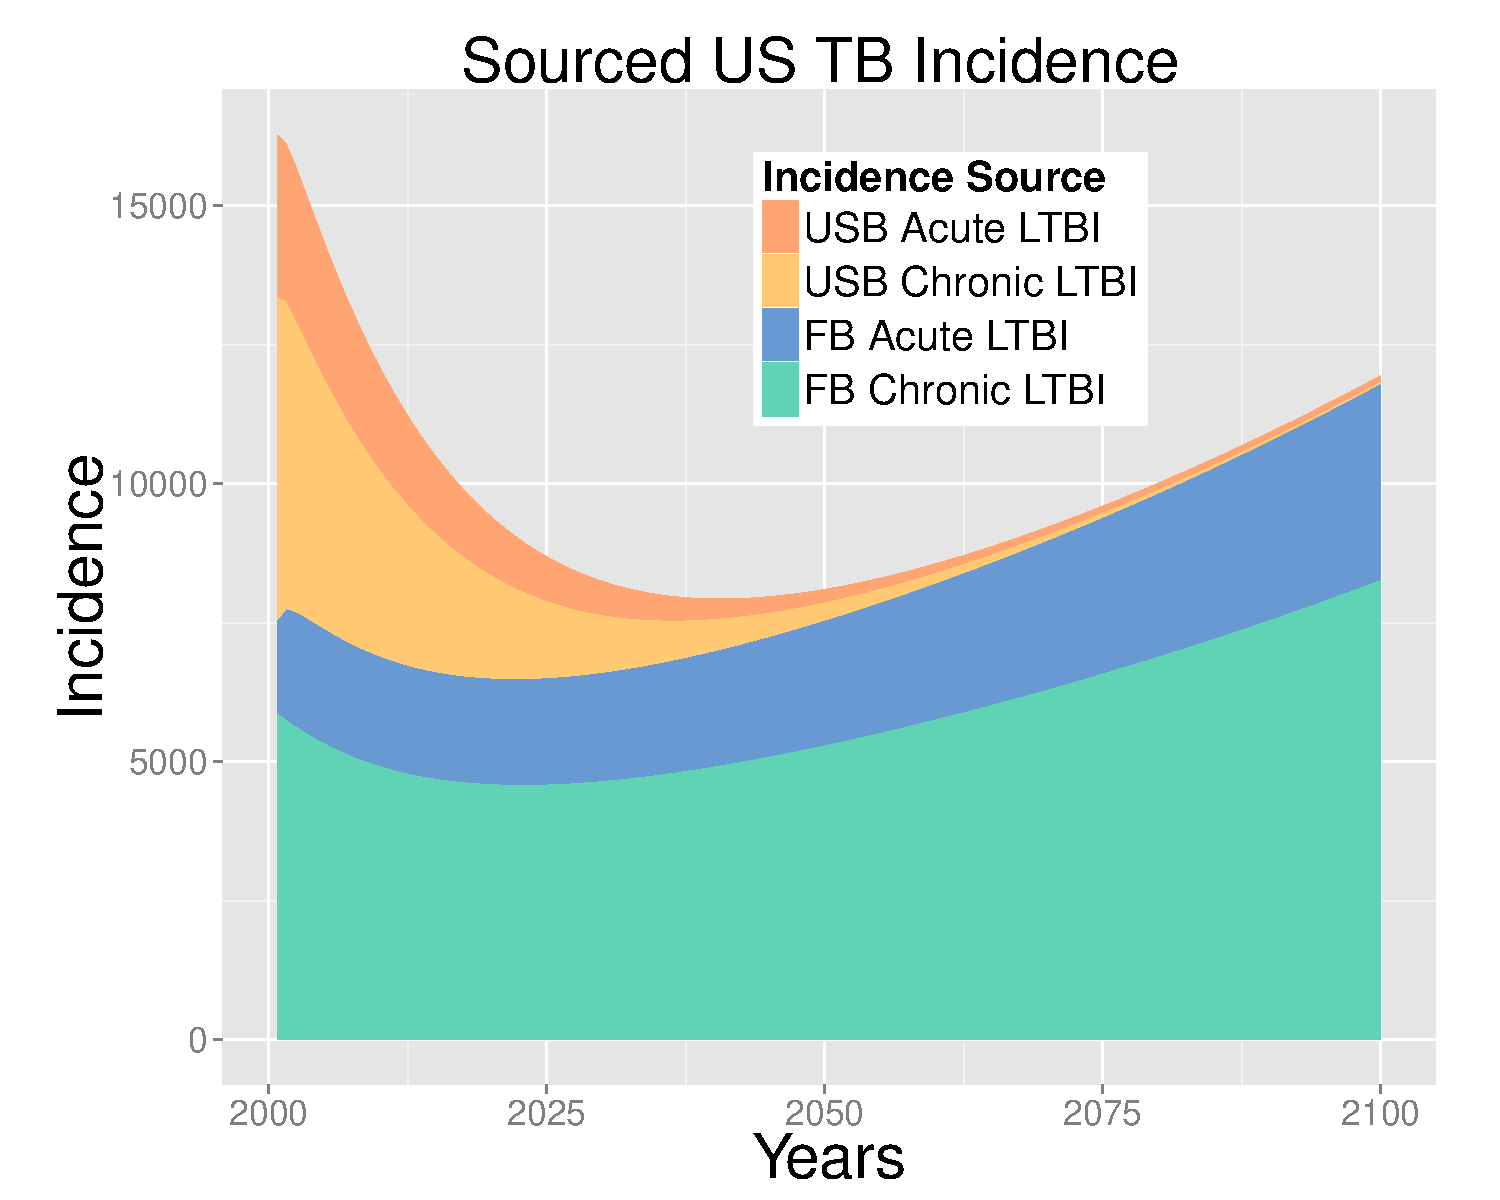
\includegraphics[scale=.5]{incPlotSourced}
  \end{center}
  \caption{Sourced yearly incidence data generated by the extended Hill Model.}
  \label{fig:incPlotSourced}
\end{figure}
Further, figure~\ref{fig:costPlotSourced} shows a similarly sourced plot, but analyzing the
final US HCS costs due to active TB. One can see that in this plot, roughly half
of the US TB HCS costs are due to activations of LTBI. Note that In this data,
it is appropriate to think of the costs due to acute LTBI as costs due to
exogenous re-inection, whereas active TB costs due to chronic LTBI are
activations of long standing latent infections into active TB. 
\begin{figure}[h]
  \begin{center}
    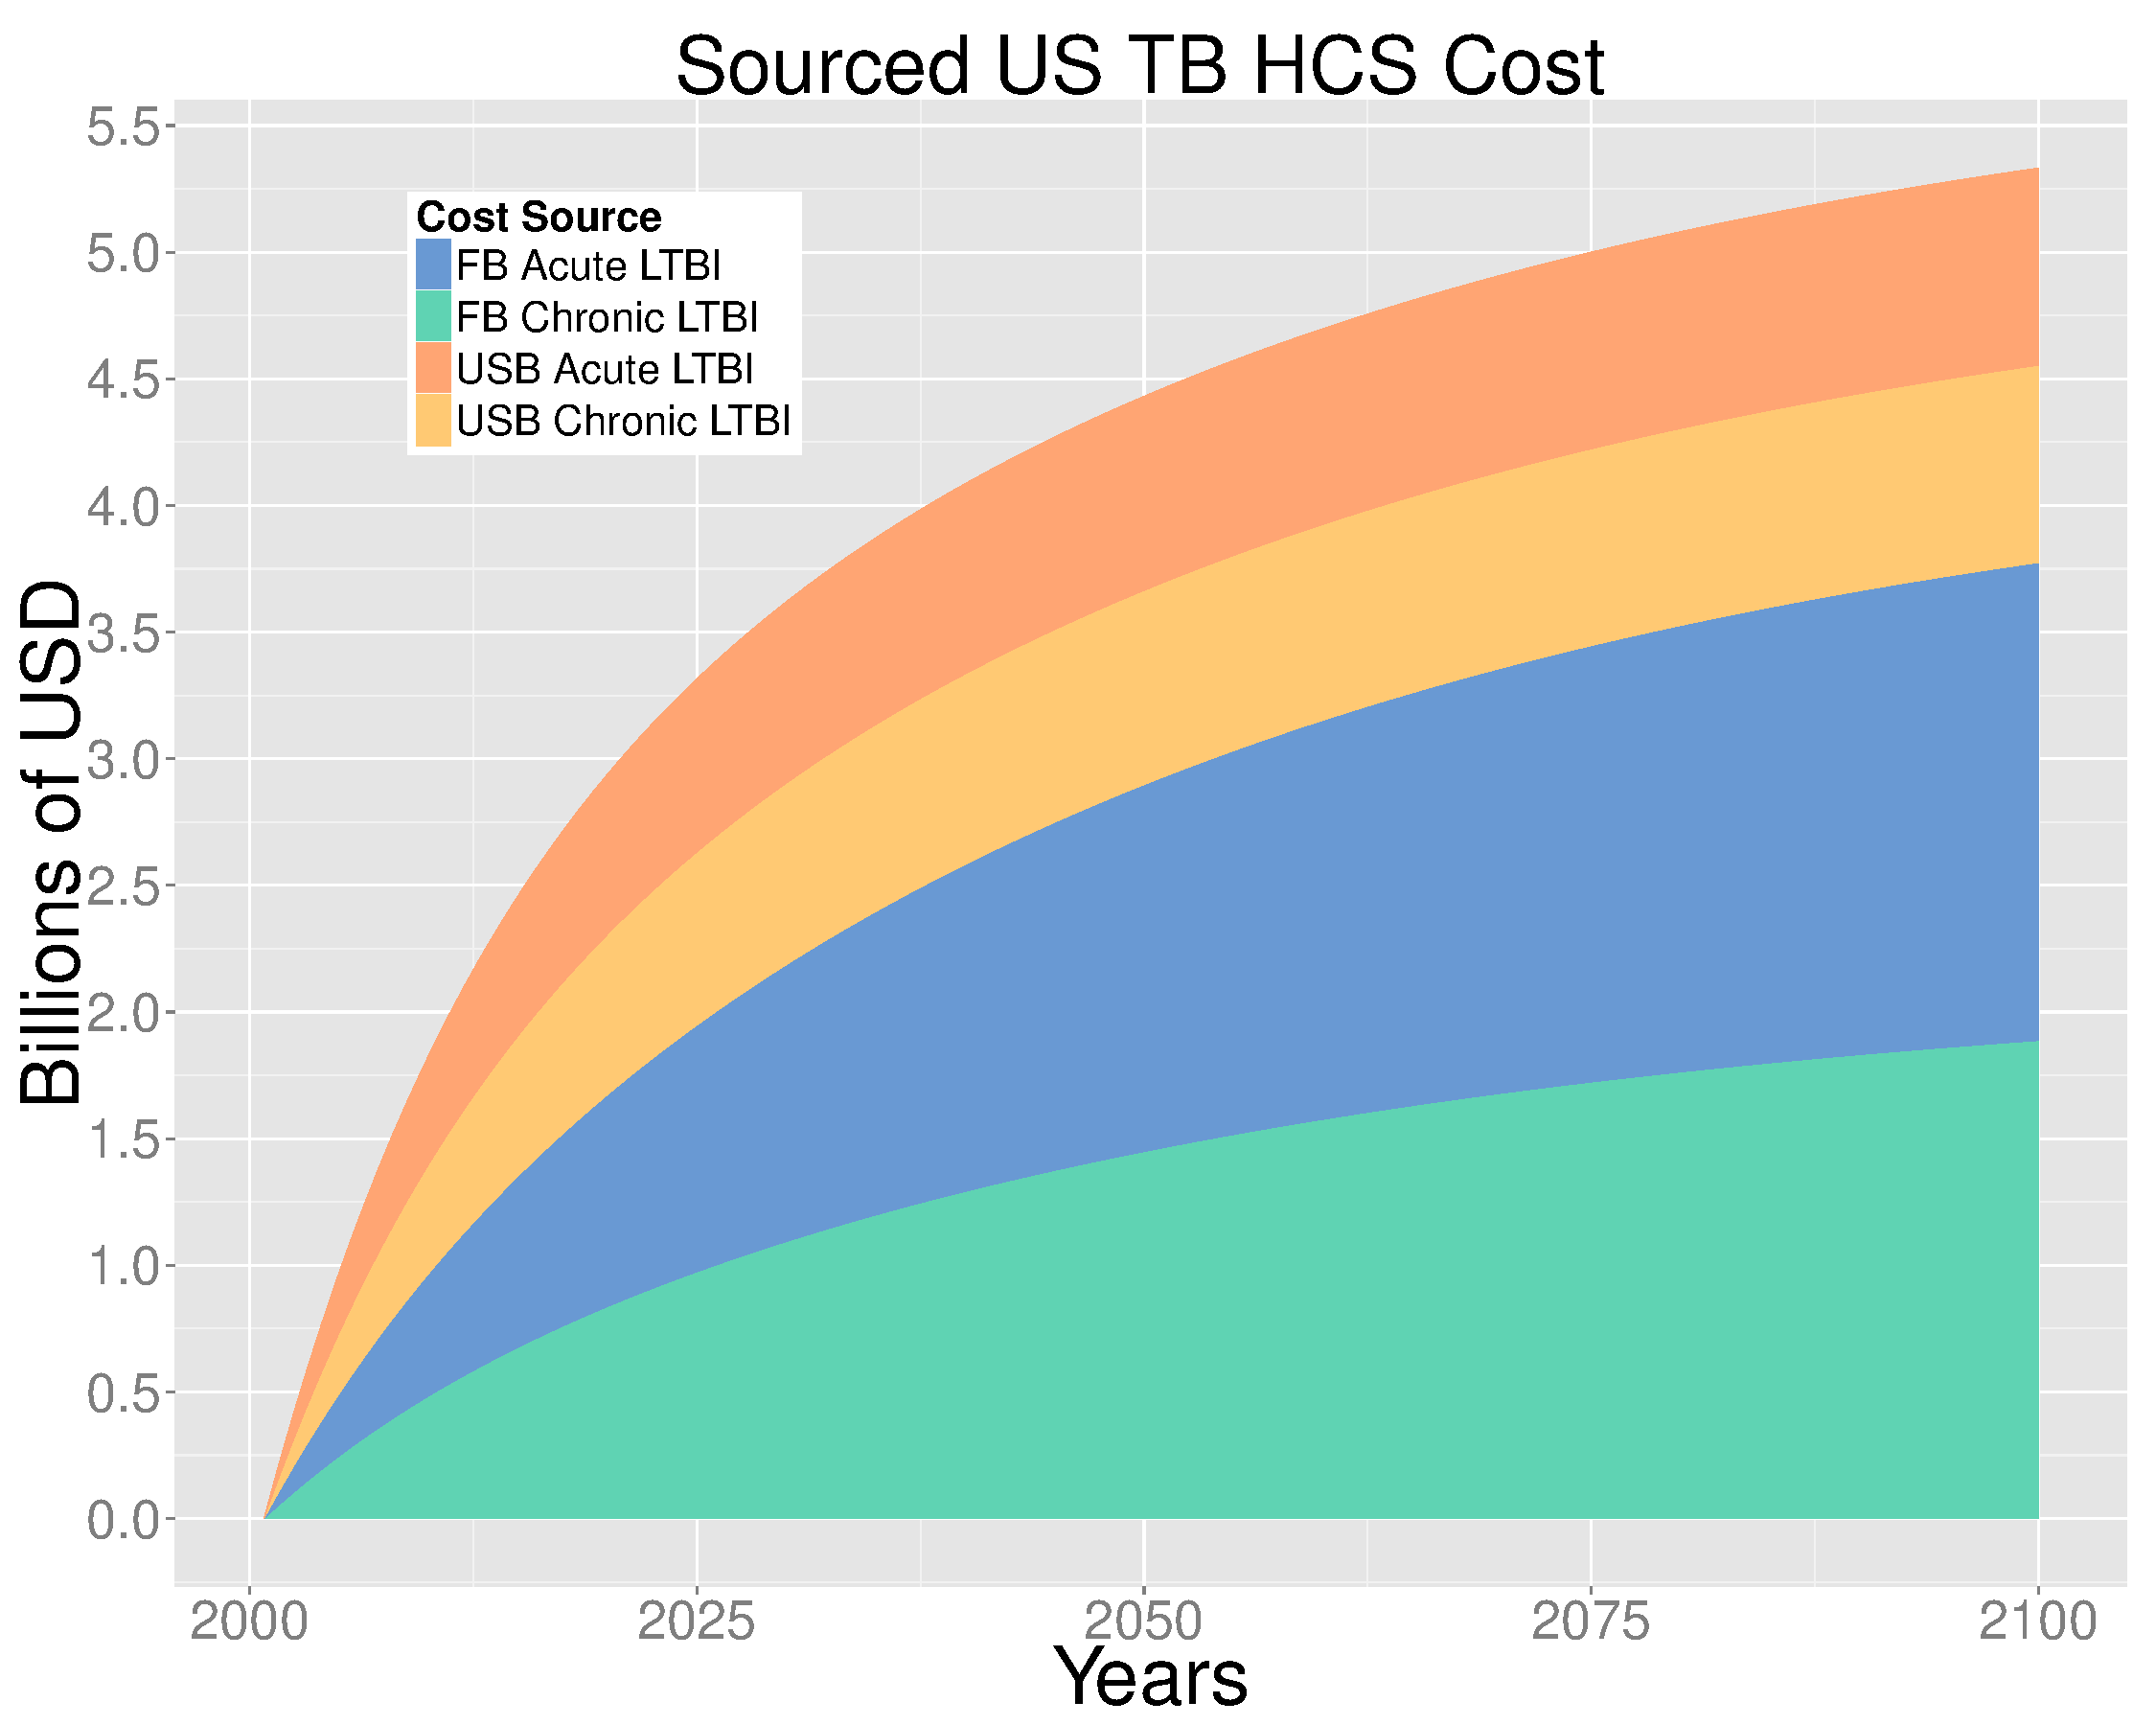
\includegraphics[scale=.35]{costPlotSourced}
  \end{center}
  \caption{Sourced US HCS economic TB load. Note that this data only illustrates
    the load due to treating active TB, but illustrates where the infections
    driving this cost come from.}
  \label{fig:costPlotSourced}
\end{figure}
Note that both of these plots underestimate the impact LTBI activations play in
the spread of TB, as every LTBI activation to infectious TB contributes not only
to incidence and costs directly, but also indirectly by causing additional
future cases, which is not captured in these graphs. Further, there are also US
HCS costs due to LTBI treatment, which is not illustrated in these graphs. 
\subsubsection{Basic Reproduction Number}
The basic reproduction number of FB or USB cases of infectious TB was also
estimated by this system. Using the best-fit values of parameters from the 
Hill model, we found the average number of secondary infections arising from
a single case of infectious TB to be 0.423 and 0.370 for USB and FB populations
respectively.  These values differ because in the model, there are different
estimates for death rates and the rate of TB treatment and self-cure in the USB and FB populations, 
so the average infectious period differs between the two populations.
Extrapolating these results, we can think of the
total number of secondary infections over 100 years due to a FB or USB
infectious TB case as describing a geometric series in a large population.
Presuming there are no overlaps in infectious contacts, if a single case of
infectious TB in either population infects $p_f, p_u$ new cases,
respectively, then we can say that over the course of 100 years, the total
number of cases infected will follow a geometric series. This analysis predicts
that over 100 years, one USB infection will lead to $1.04$ subsequent infections,
whereas one FB infection will lead to $.83$ subsequent infections. Experimentally, 
these data were also analyzed, with results of $1.03$ and $.64$, respectively. 
Full calculations are included in the Appendix.  

\subsection{Intervention Analysis}
The primary interventions analyzed by the extended Hill were those that analyzed
curing various percentages of entering LTBI cases. Four indicative percentages
chosen were $5\%$, $10\%$, $25\%$, and $50\%$. Note that the Hill model does
not distinguish documented immigration from undocumented immigration, and as
such estimates of entering LTBI cure rates higher than $50\%$ become much more
difficult to achieve. It was seen that in this model as well as in the basic
Hill, no analyzed intervention predicted elimination by 2100. In order to obtain
elimination by 2100, at least 95\% of entering LTBI cases had to be cured, which
is practically impossible. However, it was seen that curing entering cases of
LTBI resulted in a net US HCS cost per case averted of \$67,654.07 at 2025, \$28,699.15 at 2050,
and \$17,912.95 at 2100 (assuming 25\% reduction with each cure costing \$800; see Table
\ref{tab:cpcaArt} for other percentages). Given the variable nature of LTBI
treatment cost, the model code is extendible such that a user can adjust these
costs themselves to explore more specific methods of curing entering LTBI.
Further, it was also found that the relationship between total incidence at 2100
and percentage of incoming LTBI cases cured was linear, and from this estimates
were made of the yearly average US HCS savings garnered by curing one case of
entering LTBI over the time scale 2000 to 2025, 2000 to 2050, and 2000 to 2100.
This value peaked at \$1.283 billion at 2100 (25\% reduction). This illustrates
that it would be cost saving to cure cases of LTBI at the cost of \$1.283
billion ``2000'' dollars over the time period 2000-2100. These intervention
strategies also resulted in 11,900; 29,880; and 60,189 fewer cases of TB seen in
the US, and 1,025; 2,573; and 5,185 fewer TB deaths, for 10\%, 25\%, and 50\%
reduction, respectively.

% latex table generated in R 3.0.1 by xtable 1.7-1 package
% Mon Oct 14 00:36:15 2013
\begin{table}
\centering
\begin{tabular}{|r|cccc|} \hline
       & red5     & red10    & red25    & red50    \\ \hline
  %2000 & ND       & ND       & ND       & ND       \\ 
  2025 & 67908.81 & 67855.46 & 67654.07 & 67332.53 \\ 
  2050 & 28938.23 & 28878.70 & 28699.15 & 28404.13 \\ 
  2075 & 21044.88 & 20989.16 & 20820.53 & 20541.77 \\ 
  2100 & 18130.11 & 18076.11 & 17912.95 & 17642.64 \\ \hline
\end{tabular}
\caption{Cost Per Case Averted by Reducing Incoming LTBI by X percent (in dollar per case)} 
\label{tab:cpcaArt}
\end{table}

Several other intervention strategies analyzed by the Hill Model were refined
with the Extended Hill, and economic properties about each of them were tracked.
The results for these interventions, which are less effective than curing
entering LTBI cases across the board, are given in the appendix. 

\subsection{Sensitivity Analysis}
To account for uncertainty of input parameter values and to gain insight about
the most influential parameters in the model, we used Latin Hypercube Sampling
to analyze the deterministic model, implemented with the \texttt{lhs} package in
\texttt{R}.  We varied the 16 parameters from the original Hill model according
to triangular distributions centered around their best-fit values, and two
additional treatment cost parameters according to uniform distributions.  We
obtained similar results to the Hill model analyzing non-economic outcomes, as
expected for validation.  For economic outcomes, we found the parameter $f$, the
fraction of FB arrivals with LTBI, to be highly correlated with the projected
overall cost burden of TB in the United States over the next 100 years.  Another
highly influential parameter in the model was $\sigma^{L}$, the treatment rate
for chronic LTBI.  However, while increasing $\sigma^{L}$ significantly
decreases the cost burden due to Active TB treatment, it increases the cost
burden due to Latent TB treatment by a greater amount, given the model estimates
that Latent TB treament and Active TB treatment health care costs are
approximately \$700 and \$14,000 per case cured respectively.  A full
description of the Latin Hypercube Sampling analysis and tables of Partial Rank
Correlation Coefficient (PRCC) results for all parameters are given in the
Appendix, Section 7.6. 

\subsection{Agent Based Evaluation}
The agent-based model allowed the statistical properties of the system to be
analyzed and verified. In particular, it illustrated that the deterministic
Hill model provides a robust and consistent statistical measure of TB epidemic
behavior in the US conditions. We found that the distribution of incidence and
final population sizes were normal, with mean accurate to the deterministic
model and standard deviations given in table X, in the Appendix. Additionally,
the agent-based model provided a computational framework to produce
meaningful intervention results. On lab-grade, student hardware, a statistically
meaningful experiment could be run overnight, producing data in a day. This
demonstrates that this modeling strategy is feasible in this general case.

\section{Discussion}
These results confirm the hypothesis that curing incoming LTBI rates is a
necessary step towards elimination and indicate that it is a cost effective
option. \\
{\huge \color{red} Where did we show it was cost effective relative to other
interventions? Also, the section below (future work) might be better just
directly included in the discussion. Also, if we want to make this claim here we
need to include other interventions in the main body.}\\
In addition, beyond demonstrating quantitatively that this intervention strategy
is a necessary step towards US elimination, we also obtained qualitative
indications that this is the case. In every intervention we tested (see, for
example, Intervention <+ADD ME+> and <+ADD ME+> in section <+ADD ME+>) we
observed a plateauing effect, where the incidence per million stabilized after
some time and resisted further change. In particular, even when transmission was
reduced to $0\%$, we still observed this plateauing effect, which implies that
something other than active transmission was generating enough incidence to
sustain TB in an endemic state in the US population. However, when the FB LTBI
immigration was cut, this effect vanished. These results therefore support the
argument that the USB LTBI population is sufficiently large to sustain a
sizable, endemic TB-disease state in the United States provided it is
continually refueled via the entering LTBI immigrants. Thus, there is no
intervention that can ignore the LTBI population that can hope to eliminate TB
in the United States. Among those interventions that treat cases of LTBI,
targeting the immigrating LTBI requires no additional US HCS dollars beyond what
is spent now to identify the LTBI population and is therefore extremely
efficient. Additionally, our analysis shows that paying for the treatment of
these individuals is extremely cost effective {\huge \color{red} TODO: Show
this}.
\subsection{Future Work}
This work could be extended by examining different classes of interventions or
more accurately estimating intervention cost with the deterministic extended
Hill. Further work could also be done with the agent-based Hill Model, by using
it to examine the effect contact structure plays on US TB incidence levels or to
examine the effects drug-resistant TB will have on US TB dynamics. 

\section{Appendix}
\subsection{Hill Constants}
\label{subsec:hillConstants}
Below, we detail some of the relevant constants in the Basic Hill Model, and
their best-fit values. A full listing of constants used in the original Hill
Model can be found in <+CITATION HERE+>. \\
\textit{(USB = US born, FB = Foriegn born)}
\begin{align*}
  \sigma^{L} &= 0.057   &&\text{(Treatment rate for chronic LTBI)}\\
  v^{L}_{0}  &= 0.0014  &&\text{(Progression rate for reactivation in the USB
                                 population)}\\
  v^{L}_{1}  &= 0.0010  &&\text{(Progression rate for reactivation in the FB
                                 population)}\\
  f          &= 0.187   &&\text{(Fraction of FB arrivals with LTBI)}\\
  p          &= 0.103   &&\text{(Fraction of new infections which are acute)}\\
  ARI_{0}    &= 0.00030 &&\text{(2000 Annual Risk of Infection, USB)}\\
  q          &= 0.708   &&\text{(Fraction of infections progressing to infectious
                                 disease)}\\
  g          &= 0.0047  &&\text{(Fraction of FB arrivals with LTBI who are fast
                                 progressors)}\\
  \sigma^{F} &= 0.461   &&\text{(Cumulative fraction of treatment for acute
                                 infection)}\\
  r_{0}      &= 0.667   &&\text{(Fraction of cases due to reactivation in USB
                                 population)}\\
  r_{1}      &= 0.780   &&\text{(Fraction of cases due to reactivation in FB
                                 population)}\\
  \mu^{d}    &= 0.115   &&\text{(Mortality rate due to TB)}\\
  x          &= 0.111   &&\text{(Fraction of re-infected chronic LTBI moving to
                                 acute infection)}\\
  \phi       &= 0.897   &&\text{(Cumulative fraction self-cure and treatment of
                                 active disease)}\\
  e_{0}      &= 0.965   &&\text{(Fraction of preferred contacts within own
                                 population for USB)}\\
  e_{1}      &= 0.985   &&\text{(Fraction of preferred contacts within own
                                population for FB)}\\
\end{align*}
\subsection{The Extended Hill Equations}
\label{sec:extendedHillEqs}
Below, we detail some of the relevant equations used in the extended hill model.
In many cases, the equations of the Hill model were split into their component
parts, which could then be tracked separately. 

{\huge \color{red} TODO: What equations should be put in here?}

Here, a continuous discounting approximation is used to a discount rate of $3\%$
yearly, found via $discV$. In many of the differential equations, a small $c$ is
used to denote \emph{cost of}. 
\FloatBarrier
\subsection{Estimations for Infectious Rates of FB and USB}

\subsection{Statistical Qualities of the Agent Based Model}

\begin{figure}
    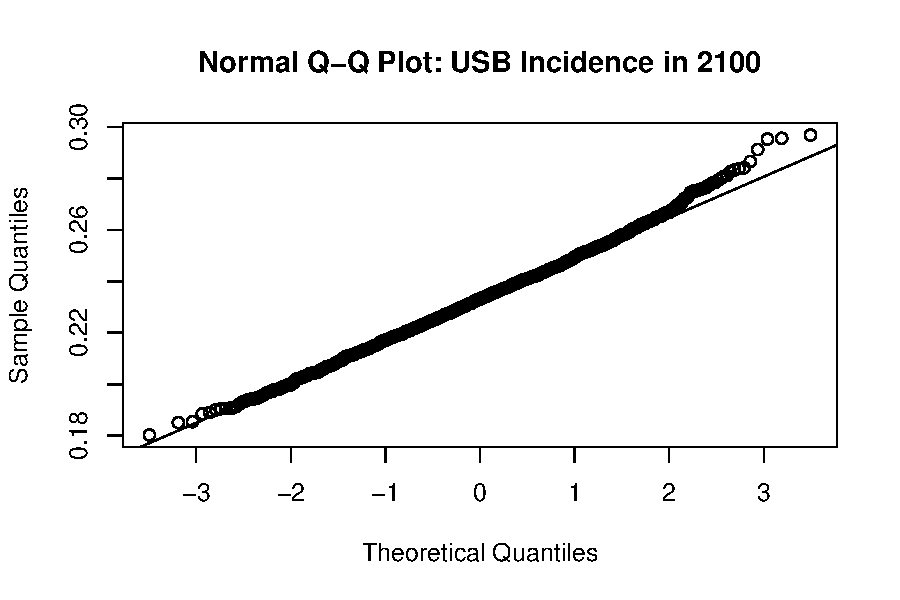
\includegraphics[scale=0.4]{figures/qqnormUSBInc.pdf}
    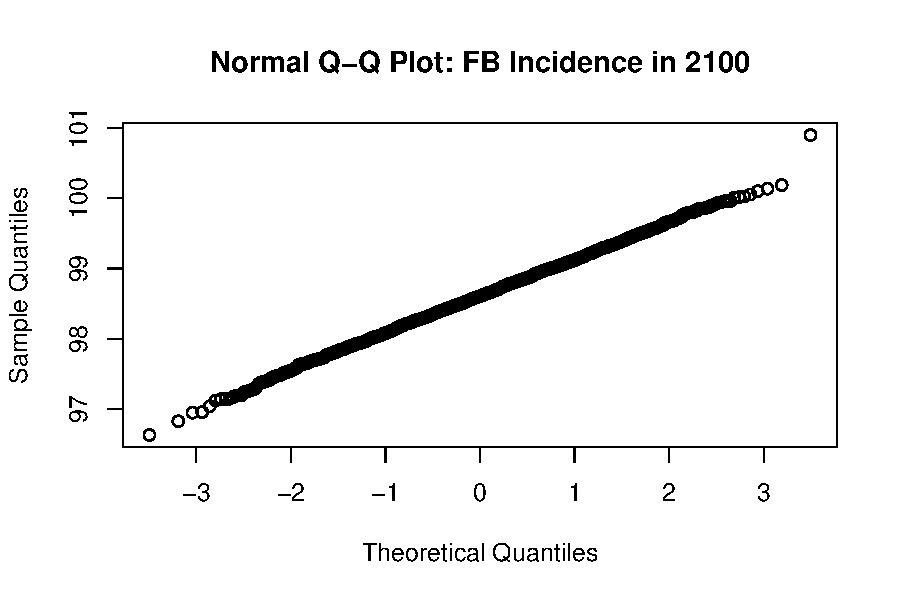
\includegraphics[scale=0.4]{figures/qqnormFBInc.pdf}
    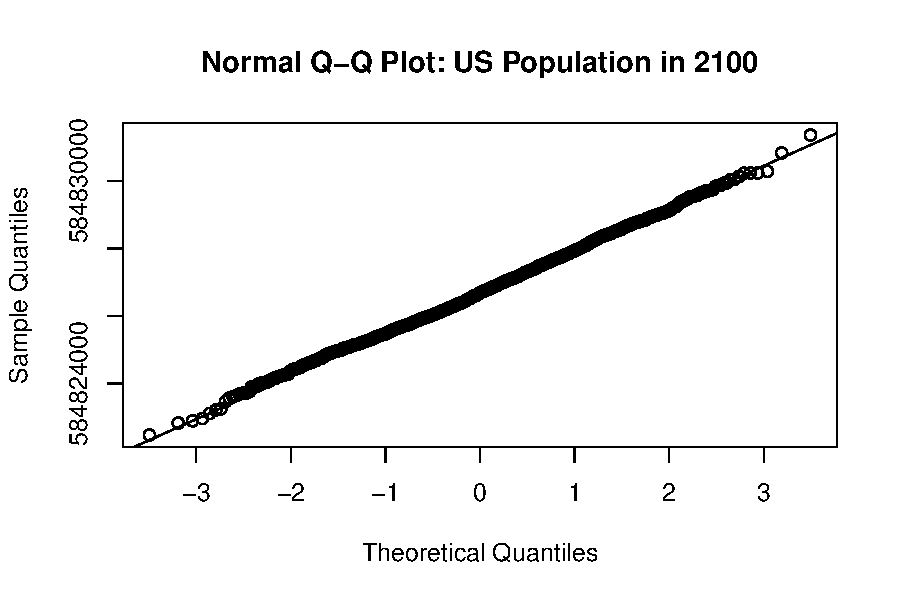
\includegraphics[scale=0.4]{figures/qqnormUSBPop.pdf}
    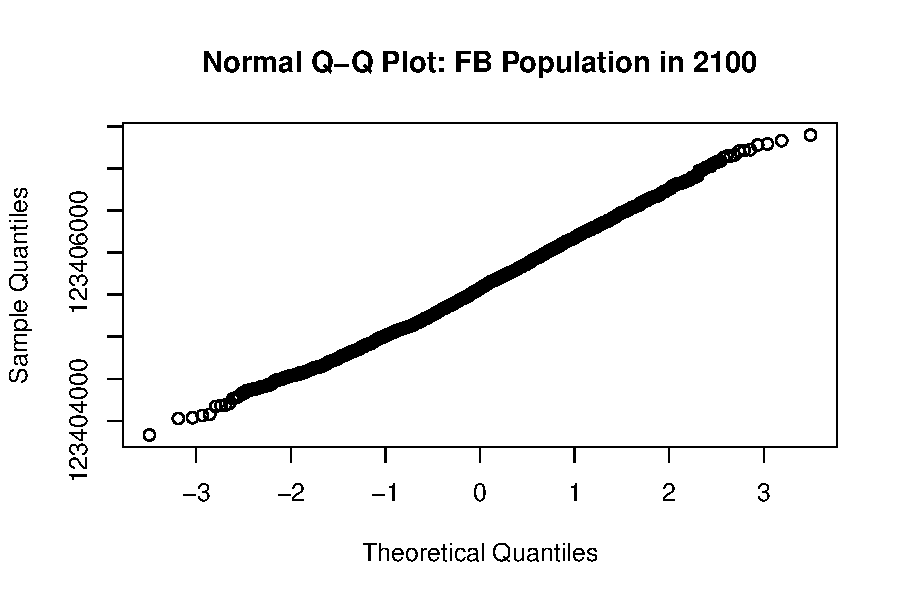
\includegraphics[scale=0.4]{figures/qqnormFBPop.pdf}
  \caption{Normal Q-Q Plots for 2103 runs of the Stochastic Model with population constant = 1.}
  \label{fig:qqnormPlots}
\end{figure}

Results for USB Incidence, FB Incidence, USB Population, and FB Population in the year
2100 shown, overlayed with linear (normal) fit are shown in
figure~\ref{fig:qqnormPlots}. These plots demonstrate the normality of the
Stocahstic Data. 
\subsection{Finer Intervention Analysis}

% latex table generated in R 3.0.1 by xtable 1.7-1 package
% Mon Oct 14 00:36:15 2013
\begin{table}
\centering
\begin{tabular}{|r|cccc|} \hline
       & red5    & red10    & red25    & red50    \\ \hline
  %2000 & 0.00    & 0.00     & 0.00     & 0.00     \\ 
  2025 & 1115.12 & 2231.70  & 5592.43  & 11227.57 \\ 
  2050 & 3406.41 & 6821.27  & 17117.18 & 34447.71 \\ 
  2075 & 4976.77 & 9967.15  & 25021.33 & 50389.58 \\ 
  2100 & 5942.02 & 11900.90 & 29880.03 & 60189.49 \\ 
   \hline
\end{tabular}
\caption{Cases of TB Averted by Reducing Incoming LTBI by various percentages
         (Cure=\$800)} 
\label{tab:caRed}
\end{table}

% latex table generated in R 3.0.1 by xtable 1.7-1 package
% Mon Oct 14 00:36:15 2013
\begin{table}
\centering
\begin{tabular}{|r|cccc|} \hline
       & red5     & red10    & red25    & red50    \\ \hline
  %2000 & ND       & ND       & ND       & ND       \\ 
  2025 & 67908.81 & 67855.46 & 67654.07 & 67332.53 \\ 
  2050 & 28938.23 & 28878.70 & 28699.15 & 28404.13 \\ 
  2075 & 21044.88 & 20989.16 & 20820.53 & 20541.77 \\ 
  2100 & 18130.11 & 18076.11 & 17912.95 & 17642.64 \\ \hline
\end{tabular}
\caption{Cost Per Case Averted by Reducing Incoming LTBI by various percent (in
dollars per case, Cure=\$800)} 
\label{tab:cpcaRed}
{\huge\color{red} We need to remake this table for Cure = $600, $1000, $1200, $1400, $1600
and put it in the appendix.}
\end{table}

\subsection{Latin Hypercube Sampling}
%The model parameters and variable names referred to in this analysis are listed
%below, along with best-fit or estimated values. 
Following the example of the
Hill model, we generated a Latin Hypercube Sample varying 18 of the input
parameters.  From these parameters, 16 are identical to the input parameters
varied in the sensitivity analysis of the original Hill model, and the remaining
two parameters, $C_{A}$ and $C_{L}$, detailed below, are variables for the average cost of
Active and Latent TB treatment in the US.   Probability distributions for the
original 16 parameters of the Hill model were all set to be Triangular, with
mode at the best fit value and end points at the 2.5 and 97.5 percentile values
reported in the Hill model.  Probability distributions for $C_{A}$ and $C_{L}$
were set to be Uniform, with range +/- 10\% of the estimated value.  All
probabilty distributions used to generate the Latin Hypercube are listed in
Table 1.\\

{\bf Additional Cost Parameters}
\begin{align*}
  C_{A} &= \$14,014.50 &&\text{(Cost per Active TB treatment)}\\
  C_{L} &= \$700       &&\text{(Cost per Latent TB treatment)}
\end{align*}
\vspace{5mm}

\begin{table}[h]
\centering
\begin{tabular}{l l}
\hline\hline\\
Parameter & Distribution\\ [0.5ex]
\hline\\
$\sigma_{L}$  & Tri(0.015,0.057,0.086) \\
$v^{L}_{1}$   & Tri(0.0009,0.0010,0.0014) \\
$f$                 & Tri(0.157,0.187,0.232) \\
$p$                & Tri(0.053,0.103,0.137) \\
$ARI_{0}$      & Tri(0.00021,0.00030,0.00030) \\
$q$                & Tri(0.569,0.708,0.825) \\
$g$                & Tri(0.0008,0.0047,0.0815)  \\
$\sigma_{F}$ & Tri(0.419,0.461,0.574) \\
$r_{1}$          & Tri(0.759,0.780,0.831) \\
$r_{0}$          & Tri(0.623,0.667,0.694) \\
$\mu^{d}$      & Tri(0.071,0.115,0.231) \\
$x$                 & Tri(0.088,0.111,0.860) \\
$v^{L}_{0}$   & Tri(0.0011,0.0014,0.0015) \\
$\phi$            & Tri(0.861,0.897,0.938) \\
$e_{0}$          & Tri(0.853,0.965,0.995) \\
$e_{1}$          & Tri(0.877,0.985,0.999) \\
$C_{A}$           & Uniform(12613,15416) \\
$C_{L}$           & Uniform(630,770) \\ [1ex]
\hline
\end{tabular}\\[1ex]

{\bf Table 1.} Probability distributions for model parameters, where Tri(x,y,z) denotes the 
Triangular distribution with endpoints (x,z) and mode y.
\end{table}

With a random Latin Hypercube Sample of size n=100,000, we computed partial rank correlation coefficients (PRCC) for each of the initial parameters and treatment costs, according to four different outcomes: 1) projected annual incidence in 2100 in the overall population, 2) projected cumulative cost of Latent TB treatments by 2100, 3) projected cumulative cost of Active TB treatments by 2100, 4) projected cumulative total cost of TB treatments by 2100.  For outcome 1, PRCC values are shown alongside PRCC values computed in the original Hill model for the same outcome in Table 2, showing the closeness of our findings to the sensitivity results of the original Hill model.  PRCC values for the remaining outcomes are reported in Table 3.  \\

\begin{table}[h]
\centering
\begin{tabular}{l r r}
\hline\hline\\
Parameter & Extended Hill Model & Original Hill model \\ [0.5ex]
\hline\\
$\sigma^{L}$  & -0.9303 & -0.9381 \\
$v^{L}_{1}$   & 0.7871  & 0.8309 \\
$f$                 & 0.7050  & 0.8072 \\
$p$                & 0.8369  & 0.6100 \\
$ARI_{0}$      & 0.5950  & 0.4939 \\
$q$                & 0.5797  & 0.4543 \\
$g$                & 0.6122  & 0.4517 \\
$\sigma^{F}$ & -0.4911 & -0.3772 \\
$r_{1}$          & 0.0028  & -0.1109 \\
$r_{0}$          & 0.0018  & 0.0760 \\
$\mu^{d}$      & 0.0923 & 0.0513 \\
$x$                 & 0.0999 & 0.0345 \\
$v^{L}_{0}$    & 0.0133 & 0.0266 \\
$\phi$             & 0.0082 & 0.0177 \\
$e_{0}$          & 0.0178 & -0.0072 \\
$e_{1}$          & 0.1154 & 0.0046 \\
$C_{A}$          & -0.0023 & N/A \\
$C_{L}$           & 0.0009 & N/A \\ [1ex]
\hline
\end{tabular}\\[1ex]

{\bf Table 2.} PRCC values for projected annual incidence in 2100
 in the overall population, alongside corresponding values from the
original Hill model.
\end{table}

From Table 2, we see that the PRCC values in the Extended Hill Model and the
Original Hill Model match up reasonably well.  In both cases, $\sigma^{L}$ is
the most influential parameter, with PRCC values around -0.93.  The cost
parameters $C_{A}$ and $C_{L}$ have PRCC values close to zero, which is expected
because varying the treatment costs should not affect the incidence rate of TB.
Parameters in the original Hill model with small PRCC magnitudes (less than
0.15) also have small PRCC values in the extended model, while parameters with
larger PRCC magnitudes (greater than 0.35) similarly have large PRCC values in
the extended model.  This validates the non-economic components of our model
against the original Hill model.   \\

\begin{table}[h]
\centering
\begin{tabular}{l r r r}
\hline\hline\\
Parameter & Latent Costs & Active Costs & Total Costs\\ [0.5ex]
\hline\\
$\sigma^{L}$ & 0.9612  & -0.9284 & 0.4169 \\
$v^{L}_{1}$  & -0.4190 & 0.6470  & 0.3533 \\
$f$          & 0.7467  & 0.5493  & 0.8083 \\
$p$          & 0.3371  & 0.8810  & 0.8776 \\
$ARI_{0}$    & 0.3920  & 0.6728  & 0.7337 \\
$q$          & 0.3837  & 0.6573  & 0.7200 \\
$g$          & 0.1120  & 0.5369  & 0.5182 \\
$\sigma^{F}$ & -0.1138 & -0.5631 &-0.5435 \\
$r_{1}$      & 0.1253  &  0.0658 & 0.1401 \\
$r_{0}$      & 0.1325  & 0.0878  & 0.1658 \\
$\mu_{d}$    & 0.0249  & 0.0560  & 0.0613 \\
$x$          & 0.0214  & 0.1282  & 0.1253 \\
$v^{L}_{0}$  & -0.3103 & 0.0502  &-0.1867 \\
$\phi$       & -0.0023 & -0.0102 &-0.0107 \\
$e_{0}$      & 0.0081  & 0.0253  & 0.0269 \\
$e_{1}$      & 0.0804  & 0.1653  & 0.1926 \\
$C_{A}$      & 0.0011  & 0.7024  & 0.6385 \\
$C_{L}$      & 0.8515  & 0.0013  & 0.7598 \\ [1ex]
\hline
\end{tabular}\\[1ex]

{\bf Table 3.} PRCC values for cumulative US Health Care system costs from 
Latent TB treatment, Active TB treatment, and Total treatment costs
\end{table}

In Table 3, we see that the cost parameters $C_{A}$ and $C_{L}$ are highly
correlated with Active treatment costs and Latent treatment costs respectively.
These high PRCC values are expected because there is a linear relationship
between $C_{A}$ and the cumulative Active treatment cost, and similarly for
$C_{L}$ and the cumulative Latent treatment cost.  In addition, we note that
both $C_{A}$ and $C_{L}$ are influential in the total overall cost, with PRCC
values of 0.6385 and 0.7598 respectively.  Because the PRCC value for $C_{L}$ is
greater here, despite the fact that $C_{A} > C_{L}$, we can infer that
cumulative Latent TB treatment costs are projected to be greater than cumulative
Active TB costs with these estimates for cost parameters, so $C_{L}$ is a more
influential parameter for total cumulative treatment costs.  

Other variables with significant PRCC magnitudes (greater than 0.5) in Table 3
include $\sigma^{L}$, $v^{L}_{1}$, $f$, $p$, $ARI_{0}$, $q$, $g$, and
$\sigma^{F}$.  Two of these parameters, $\sigma^{L}$ and $v^{L}_{1}$, have
relatively large PRCC magnitudes for both Latent and Active Costs, but smaller
PRCC magnitudes for Total Costs.  Because their PRCC values for each of these
two outcomes is different in sign, the net change to the total cost is partially
cancelled out, so these parameters have a reduced influence on final US
healthcare system costs.  On the other hand, parameters such as $f$ and $p$ have
large positive PRCC values for both Latent Costs and Active Costs, and we
observe large positive PRCC values for Total Costs as well.\\

To gain insight about strategies to reduce the cost burden for TB in the US, we
focus on the parameters with the greatest PRCC magnitudes for Total Cost aside
from $C_{A}$ and $C_{L}$, namely $f$, $p$, $ARI_{0}$, and $q$.  All these
parameters have PRCC magnitudes above 0.7, and are highly correlated with the
total cost burden of TB borne by the US projected over the next 100 years.  Out
of these, $ARI_{0}$ is based on a historical fixed value, the Annual Risk of
Infection among the US born population in the year 2000, and therefore is
unchangeable under any intervention strategy.  The parameters $p$ (the fraction
of new infections which are acute) and $q$ (the fraction of infections
progressing to infectious disease) are variables which depend on physiological
disease dynamics, and may be altered with advances in medicine or mutations in
the bacterial strains of TB.  The parameter $f$ is the fraction of FB arrivals
with LTBI, which may vary depending on US immigration policies and medical
practices.  These results suggest that treating cases of LTBI among new FB
arrivals may be the most cost efficient intervention strategy to reduce the
disease burden for TB in the US, under the assumptions of the Hill model.  \\
\end{document}
